\chapter{Protótipo de Tela}

\section{Objetivo}

Este documento tem como finalidade apresentar uma visão do design do layout onde o usuário irá controlar parte da automação da casa.

\section{Protótipo}

Um dos pricipais objetivos dos protótipos é reduzir os aspectos negativos da experiência de usuário (p.ex., frustação, aborrecimento) e ao mesmo tempo melhorar os positivos (p.ex., divertimento, compromisso) \cite{design3ed}, seguindo esse pensamento, foi elaborado protótipos visando a usabilidade e praticidade no manuseio das ferramentas de automação da casa.

\begin{figure}[!htb]
  \begin{center}
	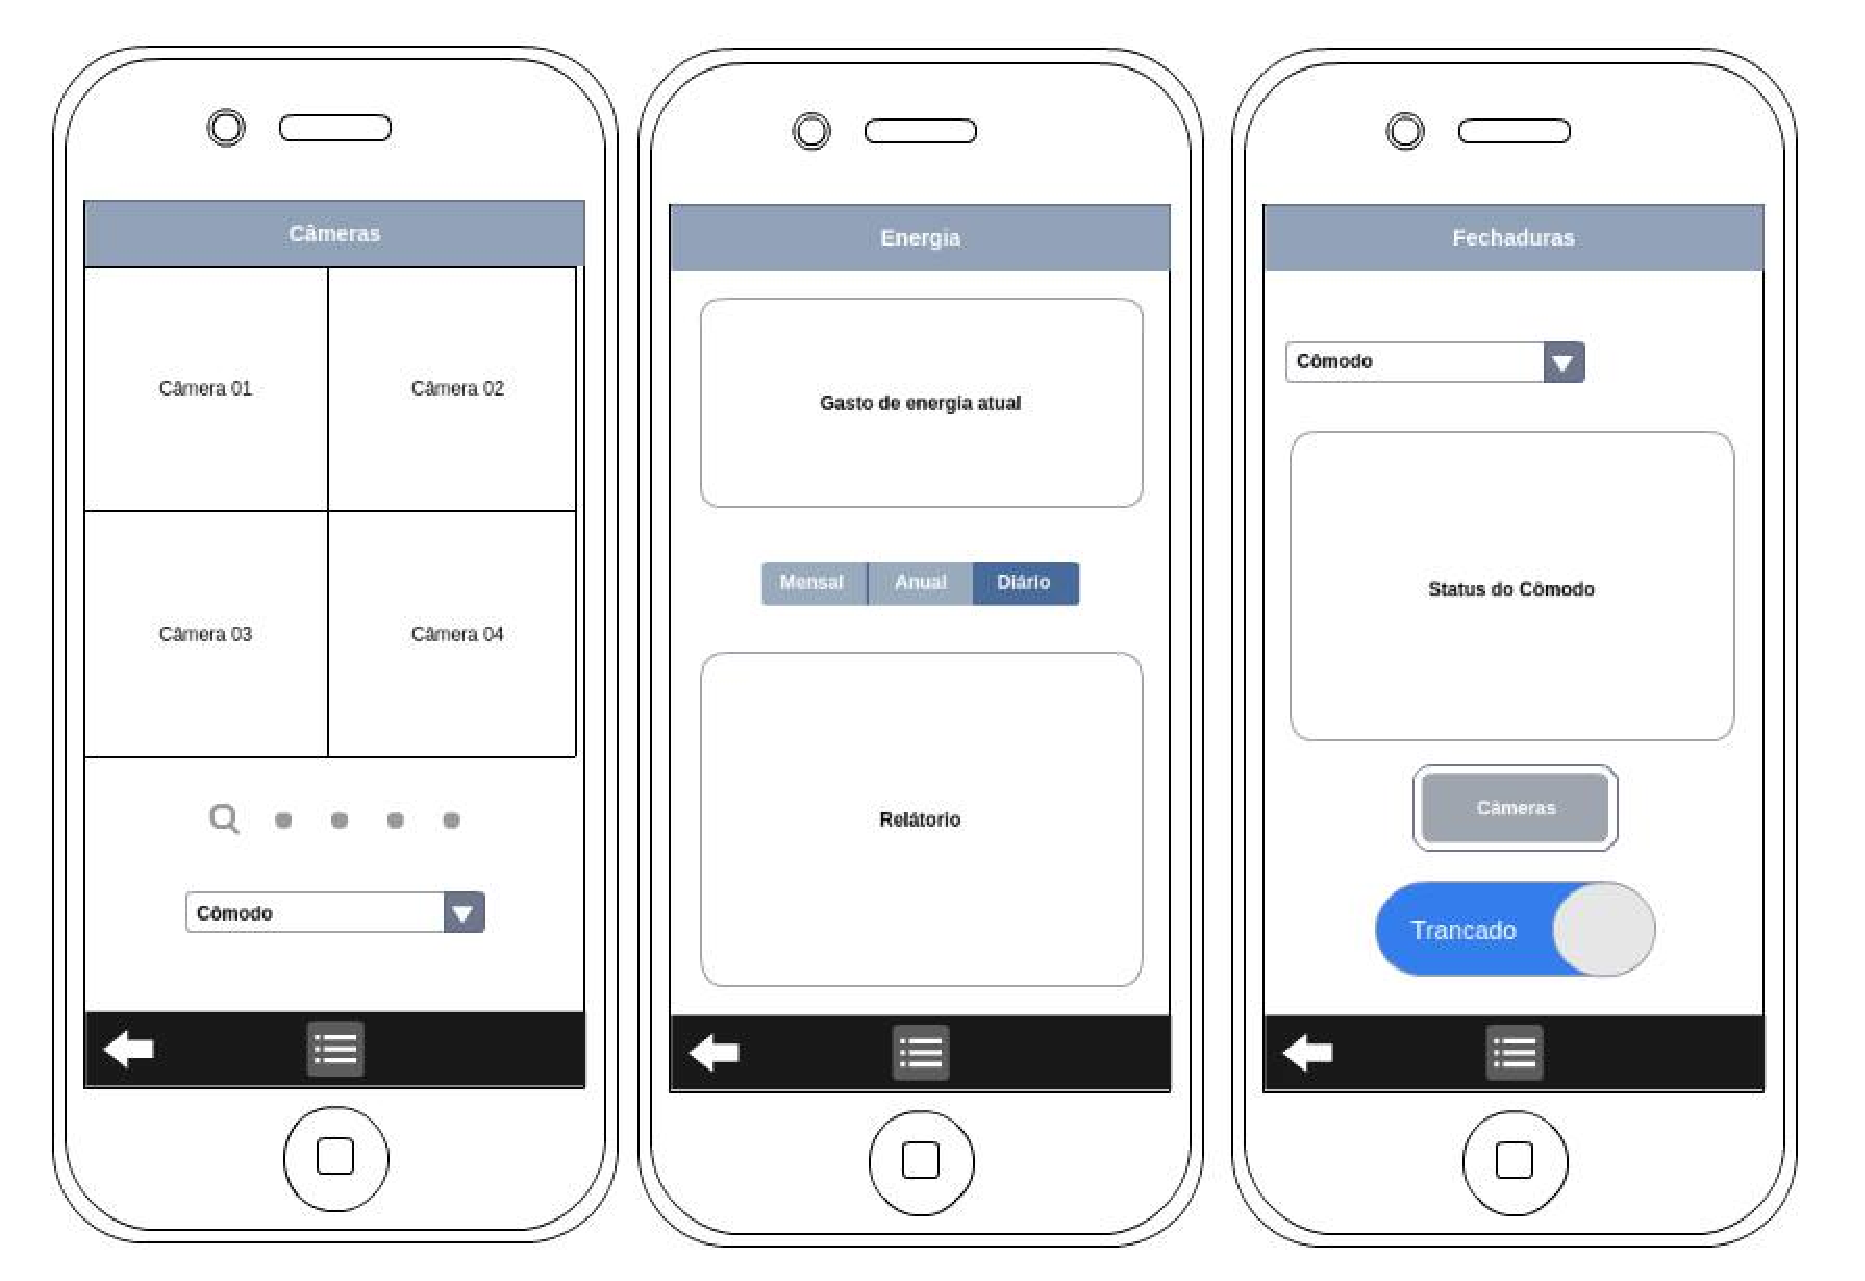
\includegraphics[keepaspectratio,scale=0.6]{figuras/prototipo1.eps}
	\caption{Protótipo de Tela}
  \end{center}
\end{figure}

\begin{figure}[!htb]
  \begin{center}
	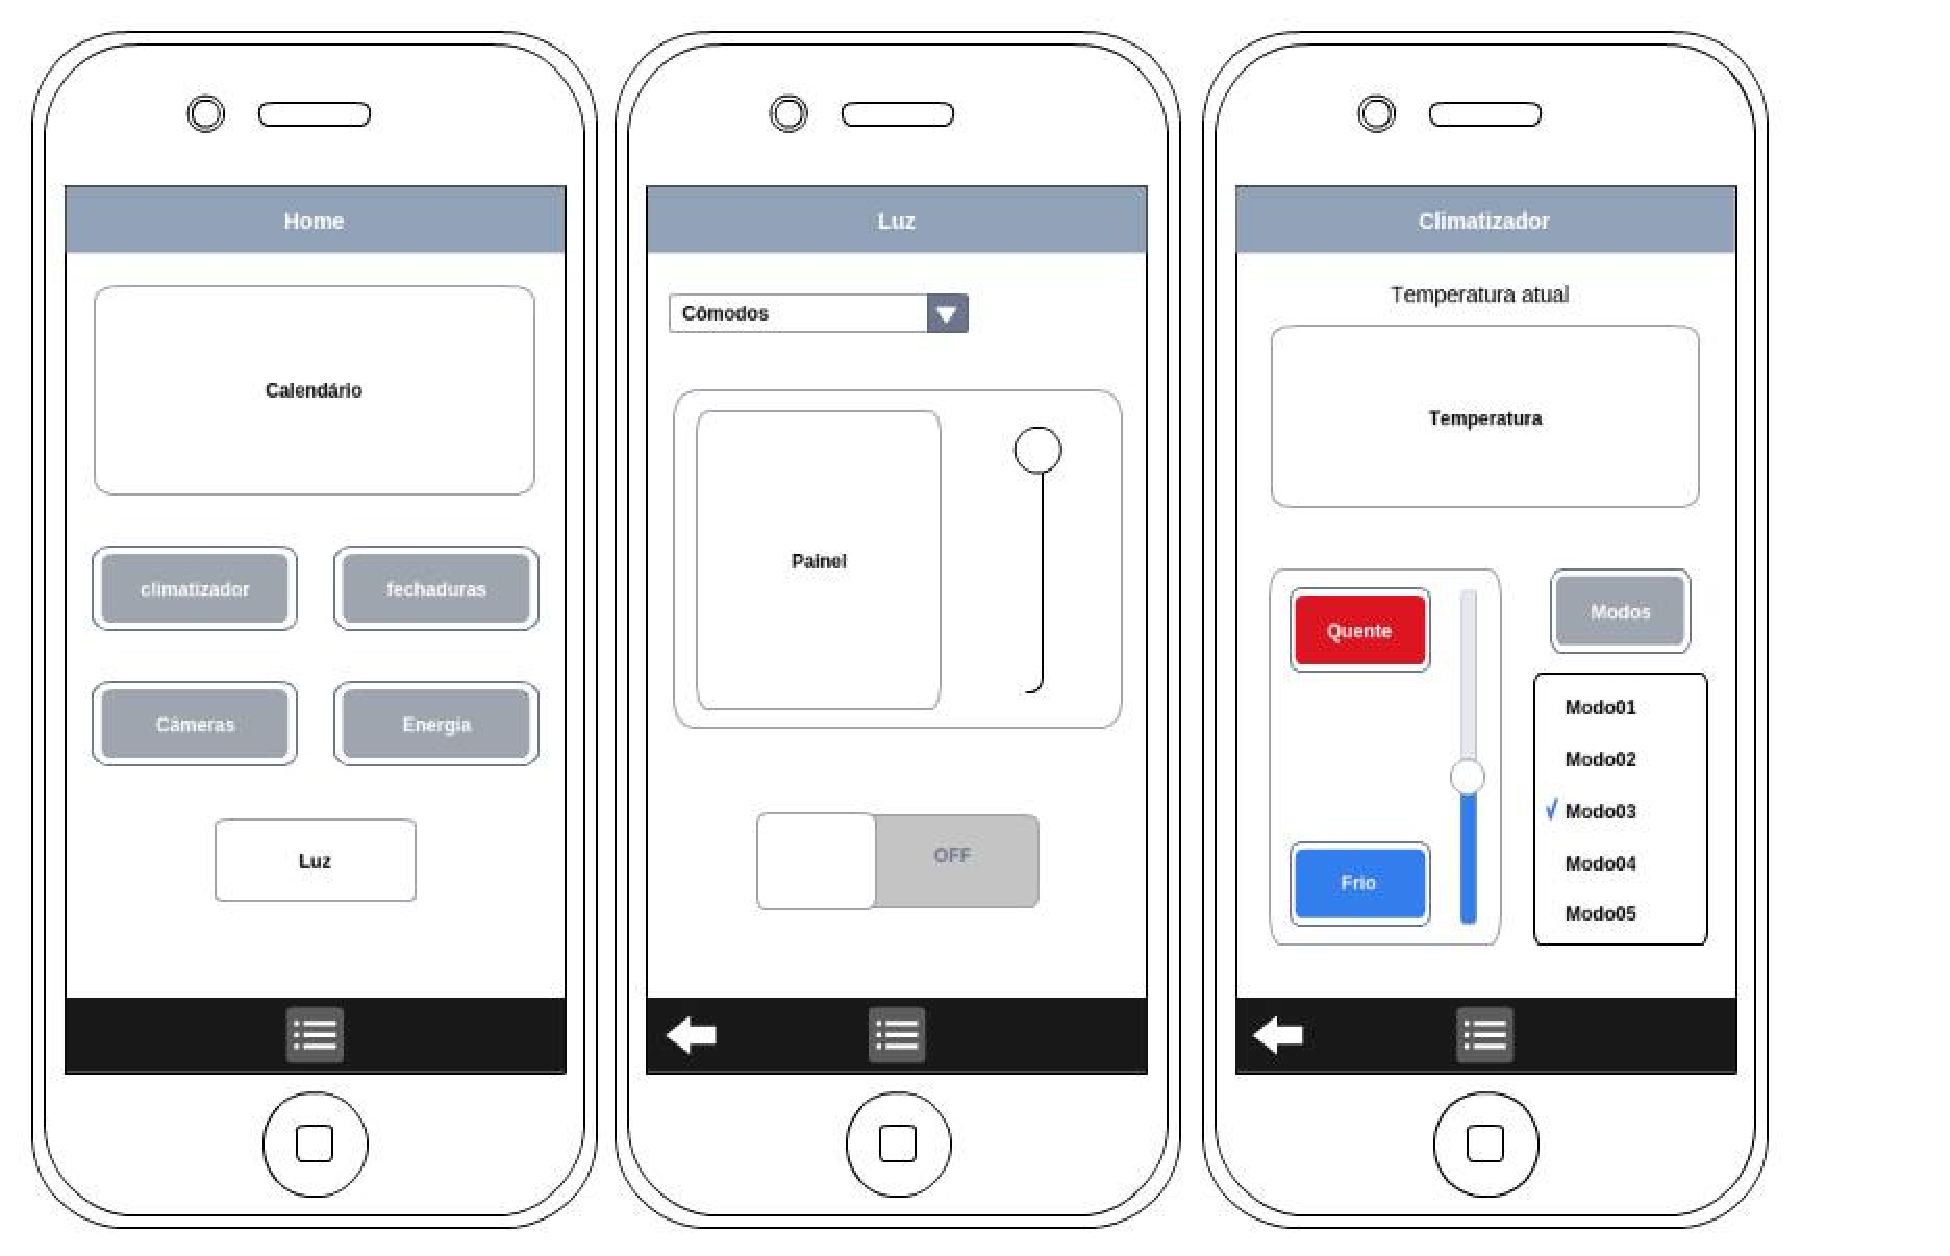
\includegraphics[keepaspectratio,scale=0.6]{figuras/prototipo2.eps}
	\caption{Protótipo de Tela}
  \end{center}
\end{figure}